\documentclass[xcolor=dvipsnames,aspectratio=169]{beamer}

% INCLUSIÓN DOS PAQUETES IMPRESCINDIBLES DE IDIOMA E CODIFICACIÓN DE CARACTERE.
\usepackage[T1]{fontenc}
\usepackage[english]{babel}
\usepackage[utf8]{inputenc}
\usepackage{csquotes}

%ACRONYMS para engadir un glosario de acronimos automatizado
% \usepackage[acronyms,nonumberlist,nopostdot,nomain,nogroupskip]{glossaries}
% \input{./acronyms.tex}

% PAQUETES PARA FIGURAS E GRAFICOS
\usepackage{graphicx}
%   \usepackage[pdftex]{graphicx}
  \usepackage{epstopdf}
   \graphicspath{{./img/}}
  % and their extensions so you won't have to specify these with
  % every instance of \includegraphics
   \DeclareGraphicsExtensions{.eps,.pdf,.png,.jpg}   
\usepackage{subfigure}
\usepackage{caption}

%Tikz plots
\usepackage{tikz}
\usepackage{tikzscale}
\usetikzlibrary{plotmarks,patterns,decorations.pathreplacing,backgrounds,calc,arrows,arrows.meta,spy,matrix,backgrounds,shapes}

\tikzset{
    block/.style = {draw, rectangle, 
        minimum height=1cm, 
        minimum width=1.2cm},
    input/.style = {coordinate,node distance=1cm},
    output/.style = {coordinate,node distance=2cm},
    arrow/.style={draw, -latex,node distance=1.5cm},
    pinstyle/.style = {pin edge={latex-, black,node distance=1.5cm}},
    sum/.style = {draw, circle, node distance=1cm}
}
\newcommand{\tikzmark}[1]{\tikz[overlay,remember picture] \UE (#1) {};}
\newcommand{\DrawBox}[4][]{%
    \tikz[overlay,remember picture]{%
        \coordinate (TopLeft)     at ($(#2)+(-0.4em,1.6em)$);
        \coordinate (BottomRight) at ($(#3)+(0.4em,-1.0em)$);
        %
        \path (TopLeft); \pgfgetlastxy{\XCoord}{\IgnoreCoord};
        \path (BottomRight); \pgfgetlastxy{\IgnoreCoord}{\YCoord};
        \coordinate (LabelPoint) at ($(\XCoord,\YCoord)!0.5!(BottomRight)$);
        %
        \draw [red,#1] (TopLeft) rectangle (BottomRight);
        \UE [below, #1, fill=none, fill opacity=1] at (LabelPoint) {#4};
    }
}
\newcommand*\circled[1]{\tikz[baseline=(char.base)]{
            \node[shape=circle,draw,inner sep=1.3pt] (char) {#1};}}
\usepackage{pgfplots}
\pgfplotsset{compat=newest}
\pgfplotsset{plot coordinates/math parser=false}
\usepgfplotslibrary{patchplots,groupplots}

% OUTROS PAQUETES DE USO COMUN. HOXE EN DIA OS COMPILADORES SON TAN RAPIDOS QUE EU METO TODOS SEMPRE
% \usepackage{float}
% \usepackage{ucs} 
% \usepackage{subcaption}
\usepackage{psfrag}
\usepackage{verbatim}
\usepackage{amsmath}
\usepackage{amsfonts} 
\usepackage{amssymb} 
\usepackage{amsthm}
\usepackage{pifont}
\usepackage{array}
\usepackage{listings}
\usepackage{stfloats}
\usepackage{algorithm} 
\usepackage{algorithmic} 
\usepackage{url} 
\usepackage{enumerate}
\usepackage{multirow}
\usepackage{wasysym}
\usepackage{cancel}
\usepackage{lmodern}
\usepackage{mathrsfs}


% DECLARACION DAS FONTES DA UVIGO
\usepackage[sfdefault]{roboto}
\usepackage{librebaskerville}
\setbeamerfont{title}{family=\librebaskerville,size=\Huge}
\setbeamerfont{subtitle}{family=\librebaskerville,size=\large}
% IMPORTANTE: a fonte 'campus' non queda ben para títulos de papers academicos,ç
% pero se de verdade se desexa empregar, seguir os seguintes pasos
% 1) Instalar o comando otftotfm en linux
% 2) sudo otftotfm -a -e texnansx campus_bold.otf CampusBold
% 3) asegurarse que o ficheiro auxiliar ./EETtemplateFiles/fonts/T1CampusBold.df está no directorio de traballo
% 4) descomentar a liña abaixo e comentar a liña que lle asigna librebaskerville arriba
\input{EETtemplateFiles/fonts/T1CampusBold.df}
\setbeamerfont{title}{family=\fontfamily{CampusBold},size=\Huge}

% DETLARACIÓN DO TEMA A USAR
% 
% ESTES TEMAS TEÑEN CABECEIRAS MOI GRANDES
% \usetheme{Berkeley} %large titlebar w/side dossier
% \usetheme{PaloAlto} 
% \usetheme{Copenhagen} %large titlebar w/2 side index
% \usetheme{Antibes} %large titlebar w/tree
% \usetheme{Singapore} %large titlebar w/balls evanescent
% \usetheme{Berlin} %large titlebar w/balls solid
% \usetheme{Dresden} %same as above with different color boxing
% \usetheme{Rochester} %large tittle-only titlebar
% ESTES TEMAS TEÑEN CABECEIRAS MEDIANAS
% \usetheme{CambridgeUS} %title titlebar w/current section
% \usetheme{Malmoe} %title titlebar w/current section Copenhagen style
% \usetheme{Madrid} %title titlebar w/page counter footer
% ESTES TEMAS TEÑEN CABECEIRAS DELGADAS
% \usetheme{Frankfurt} %small titlebar w/ progress balls
% \usetheme{metropolis} %metal
% ESTES TEMAS NON TEÑEN CABECEIRA DE COR, PERO SI TITULO SOBRE BRANCO
% \usetheme{Boadilla} %sombras e decoracion
\usetheme{Pittsburgh} %rectangulos planos
% ESTES TEMAS TEÑEN INDICES OU INFO NUNHA BARRA LATERAL GRANDE
% \usetheme{Goettingen} %right dossier evanescent
% \usetheme{Marburg} %right dossier fading to black
% \usetheme{Bergen} %notebook

%aspect modifiers
\useinnertheme{circles} %this makes item lists nicer
% \useoutertheme{infolines} %toggle thin info borders


% DECLARACIÓN DA COMBINACIÓN DE CORES A USAR. SE NON SE ESPECIFICA NADA TOMA A DEFINIDA POR DEFECTO
\definecolor{EETblue}{HTML}{0094e0} % a mate dark blue
\usecolortheme[named=EETblue]{structure} % EET UVigo blue
% outros temas de cores de beamer
% \usecolortheme{seagull} %makes title boxes gray color with blackr
% \usecolortheme{spruce} %makes title boxes pastel blue - gray color
% cores internos (items)
% \usecolortheme[named=Red]{structure} 
% \usecolortheme[named=Green]{structure} 
% \usecolortheme[named=OliveGreen]{structure} 
% \usecolortheme[named=PineGreen]{structure} 
% \usecolortheme[named=TealBlue]{structure} 
% \usecolortheme[named=SeaGreen]{structure}
% \usecolortheme[RGB={00,78,135}]{structure} % a dark cobalt blue 
% \usecolortheme[RGB={155,0,20}]{structure} % a slighlty darkened mate red

% MODIFICACIONS DAS CORES PARA A PAXINA DE TITULO SIMILAR Á OFICIAL
\setbeamercolor*{title}{use=structure,fg=structure.bg, bg=structure.fg}  
\setbeamercolor*{subtitle}{use=structure,fg=white}  
\setbeamercolor*{author}{use=structure,fg=structure.fg}
% \setbeamercolor*{institute}{use=structure,fg=structure.fg}
\setbeamercolor*{date}{use=structure,fg=structure.fg}
\setbeamertemplate{frametitle}[default][left]

% MODIFICACIONS DA SIDEBAR E FOOTLINE PARA INCLUIR AS IMAXES CORPORATIVAS.
\setbeamertemplate{footline}[text line]{%
  \parbox{\linewidth}{
    %ESTE TEXTO DA FOOTLINE PODESE MODIFICAR A GUSTO -----------------------------------------
    \insertshorttitle\hfill\insertshortauthor\hfill\insertpagenumber / \inserttotalframenumber
    %----------------------------------------------------------------------------------------
    \hfill
  
\includegraphics[width=.15\paperwidth,trim={0 2.5cm 3.5cm .75cm},clip]{EETtemplateFiles/img/Logotipo_ESCOLA.pdf}\vspace*{2pt}}}
\setbeamersize{sidebar width left = .10\paperwidth}
\setbeamertemplate{sidebar canvas left}{}
\setbeamertemplate{sidebar left}{%
  \vspace*{\fill}
  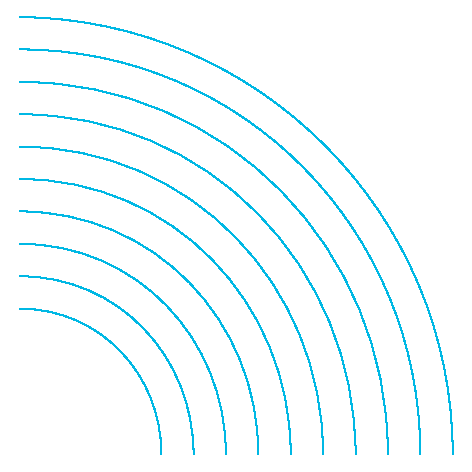
\includegraphics[width=.15\paperwidth,height=.15\paperwidth]{EETtemplateFiles/img/Simbolo_ESCOLA.pdf}\\
  
\includegraphics[width=.15\paperwidth,trim={.4cm .5cm .4cm 2.25cm},clip]{EETtemplateFiles/img/Logotipo_ESCOLA.pdf}
  \vspace*{-11pt}%
}

% MATH SYMBOLS

\newcommand{\field}[1]{\mathbb{#1}}

\DeclareMathOperator{\atan}{atan}
\DeclareMathOperator{\acos}{acos}
\DeclareMathOperator{\asin}{asin}

% \newcommand{\mb}[1]{\mathbf{#1}}


\newcommand{\Hb}{\mathbf{H}}
\newcommand{\Sb}{\mathbf{\boldsymbol{\Sigma}}}
\newcommand{\Sm}{\mathbf{S}}
\newcommand{\U}{\mathbf{U}}
\newcommand{\F}{\mathbf{F}}
\newcommand{\V}{\mathbf{V}}
\newcommand{\A}{\mathbf{A}}
\newcommand{\B}{\mathbf{B}}
\newcommand{\Cb}{\mathbf{C}}
\newcommand{\D}{\mathbf{D}}
% \newcommand{\E}{\mathbf{E}}
\newcommand{\Gb}{\mathbf{G}}
\newcommand{\T}{\mathbf{T}}
\newcommand{\I}{\mathbf{I}}
\newcommand{\Y}{\mathbf{Y}}
\newcommand{\M}{\mathbf{M}}
\newcommand{\N}{\mathbf{N}}
\newcommand{\W}{\mathbf{W}}
\newcommand{\Z}{\mathbf{Z}}
\newcommand{\R}{\mathbf{R}}
\newcommand{\K}{\mathbf{K}}
\newcommand{\X}{\mathbf{X}}
\newcommand{\Pb}{\mathbf{P}}
\newcommand{\Lb}{\mathbf{L}}
\newcommand{\Phib}{\mathbf{\boldsymbol{\Phi}}}
\newcommand{\Upsb}{\mathbf{\boldsymbol{\Upsilon}}}
\newcommand{\Delb}{\mathbf{\boldsymbol{\Delta}}}
\newcommand{\Xib}{\mathbf{\boldsymbol{\Xi}}}
\newcommand{\Q}{\mathbf{Q}}
% \newcommand{\D}{\mathbf{D}}
\newcommand{\one}{\mathbf{1}}
\newcommand{\zero}{\mathbf{0}}
\newcommand{\Rm}{\mathbf{R^{-1}}}
\newcommand{\LL}{\mathbf{\boldsymbol{\Lambda}}}
\newcommand{\J}{\mathbf{J}}

\newcommand{\ab}{\mathbf{a}}
\newcommand{\bb}{\mathbf{b}}
\newcommand{\cc}{\mathbf{c}}
\newcommand{\dd}{\mathbf{d}}
\newcommand{\e}{\mathbf{e}}
\newcommand{\f}{\mathbf{f}}
\newcommand{\g}{\mathbf{g}}
\newcommand{\h}{\mathbf{h}}
\newcommand{\m}{\mathbf{m}}
\newcommand{\n}{\mathbf{n}}
\newcommand{\pp}{\mathbf{p}}
\newcommand{\q}{\mathbf{q}}
\newcommand{\rr}{\mathbf{r}}
\newcommand{\s}{\mathbf{s}}
\newcommand{\uu}{\mathbf{u}}
\newcommand{\vv}{\mathbf{v}}
\newcommand{\w}{\mathbf{w}}
\newcommand{\x}{\mathbf{x}}
\newcommand{\y}{\mathbf{y}}
\newcommand{\z}{\mathbf{z}}
\newcommand{\al}{\mathbf{\boldsymbol{\alpha}}}
\newcommand{\vmu}{\mathbf{\boldsymbol{\mu}}}
\newcommand{\vlambda}{\mathbf{\boldsymbol{\lambda}}}
\newcommand{\vphi}{\mathbf{\boldsymbol{\phi}}}
\newcommand{\vrho}{\mathbf{\boldsymbol{\rho}}}
\newcommand{\vups}{\mathbf{\boldsymbol{\upsilon}}}

\newcommand{\rank}{\textnormal{rank}}
% \newcommand{\trace}{\textnormal{trace}}
\newcommand{\exptr}{\textnormal{exptr}}
\newcommand{\tr}{\textnormal{tr}}
\newcommand{\vstack}{\textnormal{vec}}
\newcommand{\diag}{\textnormal{diag}}
%  |x>
\newcommand{\ket}[1]{\left\vert#1\right\rangle}
%  <x|
\newcommand{\bra}[1]{\left\langle#1\right\vert}
%  <x|y>
\newcommand{\braket}[2]{\left< #1 \vphantom{#2}\,
                        \right\vert\left.\!\vphantom{#1} #2 \right>}
%  <x|a|y>
\newcommand{\sandwich}[3]{\left< #1 \vphantom{#2 #3} \right|
                          #2 \min\left(\vphantom{#1 #2} #3 \right>}

\newcommand{\pd}[2]{\frac{\partial #1}{\partial #2}}
%  d/dt
\newcommand{\ddt}{\frac{d}{dt}}
%  D/Dx
\newcommand{\pdd}[1]{\frac{\partial}{\partial#1}}
%  |x|
\newcommand{\abs}[1]{\left\vert#1\right\vert}
%  k_{x}
\newcommand{\kv}[1]{\mathbf{k}_{#1}}
%  \textnormal{E}_{domain of integration}{variable}
\newcommand{\Ex}[2]{{\mathbb{E}_{#1}\left[#2\right]}}
\newcommand{\CEx}[3]{{\mathbb{E}_{#1}\left[#2|#3\right]}}
\newcommand{\CInf}[3]{{\textnormal{I}\left(#1;#2|#3\right)}}
\newcommand{\Inf}[2]{{\textnormal{I}\left(#1;#2\right)}}
\newcommand{\CEnt}[2]{{\textnormal{H}\left(#1|#2\right)}}
\newcommand{\Ent}[1]{{\textnormal{H}\left(#1\right)}}
\newcommand{\dCEnt}[2]{{\textnormal{h}\left(#1|#2\right)}}
\newcommand{\dEnt}[1]{{\textnormal{h}\left(#1\right)}}

\newcommand{\cmark}{\ding{51}}%
\newcommand{\xmark}{\ding{55}}%
\newcommand\Tau{\mathcal{T}}
%Figure and format fixes


\renewcommand{\figurename}{Fig.}
\newcommand{\PESrule}{\noindent\rule{.57\columnwidth}{0.1mm}}

% A command to make itemized table contents

%theroem environments
% If using amsthm package, we need to delete these theorems before giving them our own definition. does not work for theorem
% \let\theorem\relax
\let\definition\relax
\let\lemma\relax
\let\corollary\relax
\let\example\relax
%
% \newtheorem{theorem}{Theorem}
\newtheorem{definition}{Definition}
\newtheorem{lemma}{Lemma}
\newtheorem{corollary}{Corollary}
\newtheorem{conjecture}{Conjecture}
\newtheorem{example}{Example}
\theoremstyle{plain}
\newtheorem{remark}{Remark}
\newtheorem{proposition}{Proposition}
   \newtheorem{homework}{Homework}

%Colors
   \definecolor{blueH3}{rgb}{0,.5,1}
   \definecolor{blueH2}{rgb}{0,0.25,0.75}
   \definecolor{blueH1}{rgb}{0,0,0.5}   
   \definecolor{grayOldText}{rgb}{.5,.5,.5}
   \definecolor{VCobalt}{HTML}{005682}
   \definecolor{TZTeal}{HTML}{008080}
   \definecolor{TZTealfaded}{HTML}{F0FFFF}
   \definecolor{KYJade}{HTML}{008151}
   \definecolor{ARust}{HTML}{a10000}
   \definecolor{FFucsia}{HTML}{7000c3}   
   \definecolor{TAMustard}{HTML}{a1a100}
   \definecolor{Tangerine}{HTML}{d45500}
   
   %%%%%%%%%%%%%%%%%%%%%%%%%%%%%%%%%%%%%%%%%%%%%%%%%%%%%%%%%%%%%%%%%
%% The following definitions are to extend the LaTeX algorithmic 
%% package with SWITCH statements and one-line structures.
%% The extension is by 
%%   Prof. Farn Wang 
%%   Dept. of Electrical Engineering, 
%%   National Taiwan University. 
%% 
\newcommand{\SWITCH}[1]{\STATE \textbf{switch} (#1)}
\newcommand{\ENDSWITCH}{\STATE \textbf{end switch}}
\newcommand{\CASE}[1]{\STATE \textbf{case} #1\textbf{:} \begin{ALC@g}}
\newcommand{\ENDCASE}{\end{ALC@g}}
\newcommand{\CASELINE}[1]{\STATE \textbf{case} #1\textbf{:} }
\newcommand{\DEFAULT}{\STATE \textbf{default:} \begin{ALC@g}}
\newcommand{\ENDDEFAULT}{\end{ALC@g}}
\newcommand{\DEFAULTLINE}[1]{\STATE \textbf{default:} }
%% 
%% End of the LaTeX algorithmic package extension.

\newcounter{MYtempeqncnt}


%%%%%%%%%%%%%%%%%%%%%%%%%%%%%%%%%%%%%%%
% Commands to recall text later
%%%%%%%%%%%%%%%%%%%%%%%%%%%%%%%%%%%%%%%
\makeatletter
\newcommand\remembertext[2]{% #1 is a key, #2 is the text
  \immediate\write\@auxout{\unexpanded{\global\long\@namedef{mytext@#1}{#2}}}%
  #2%
}
%
\newcommand\recalltext[1]{%
  \ifcsname mytext@#1\endcsname
    \@nameuse{mytext@#1}%
  \else
    ``??''
  \fi
}

%%%%%%%%%%%%%%%%%%%%%%%%%%%%%%%%%%%%%%%%%%%%%%%%%%%%%%%%%%%%%%%%%%%%%%%%%%%%%%%%%%
%%% Paolo Casari: macros for automating section titling and comment formatting %%%
%%%%%%%%%%%%%%%%%%%%%%%%%%%%%%%%%%%%%%%%%%%%%%%%%%%%%%%%%%%%%%%%%%%%%%%%%%%%%%%%%%
\newcounter{myequationcnt}

\newcounter{rcnt}
\newcounter{ccnt}

\newcommand{\newreviewernopagebreak}[1]{\vspace{5em} \setcounter{ccnt}{0}\section*{\normalsize Comments of #1}\vspace{4mm}}

\newcommand{\ThisIsTheEditorNoPageBreak}{\setcounter{ccnt}{0}\section*{\Large Comments of the Editor}\vspace{3mm}}
\newcommand{\ThisIsTheEditor}{\clearpage \ThisIsTheEditorNoPageBreak}
\newcommand{\ThisIsANewReviewerNoPageBreak}[1]{\vspace{5em} \refstepcounter{rcnt}\label{r#1}\setcounter{ccnt}{0}\section*{\Large Comments of Reviewer \arabic{rcnt}}\vspace{3mm}}
\newcommand{\ThisIsANewReviewer}[1]{\clearpage\vspace{-5em} \ThisIsANewReviewerNoPageBreak{#1}}

\newcommand{\edcomment}[1]{
\begin{tcbremark}
\color{VCobalt}
    \refstepcounter{ccnt}\label{e\arabic{ccnt}}\noindent\textbf{\boldmath\emph{Comment E.\arabic{ccnt}:}} #1\vspace{0.2cm}
\end{tcbremark}
}
\newcommand{\refedcomment}[1]{E.\ref{e#1}}

\newcommand{\revcomment}[1]{
\begin{tcbremark}
\color{VCobalt}
\refstepcounter{ccnt}\label{r\arabic{rcnt}c\arabic{ccnt}}\noindent\textbf{\boldmath\emph{Comment \arabic{rcnt}.\arabic{ccnt}:}} #1\vspace{0.2cm}
\end{tcbremark}
}
\newcommand{\refrevcomment}[2]{\ref{r#1}.\ref{r#1c#2}}

% \newcommand{\ouranswer}[1]{\noindent\emph{Answer:} #1\vspace{0.6cm}}
% \newcommand{\citepap}[1]{\vspace{0.33cm}\begin{minipage}{0.05\textwidth} $\phantom{A}$  \end{minipage}\begin{minipage}{0.85\textwidth}\renewcommand{\baselinestretch}{1.15}\small \emph{#1} \end{minipage}\vspace{0.3cm}}

\newlength{\ansspace}
\addtolength{\ansspace}{0.6cm}
\newcommand{\ansbreak}{\vspace{\ansspace}}

\newlength{\stdleftskip}
\addtolength{\stdleftskip}{\leftskip}
\newlength{\stdrightskip}
\addtolength{\stdrightskip}{\rightskip}
\newlength{\citeskip}
\addtolength{\citeskip}{2em}
\newcommand{\oldbaselinestretch}{1.5}

\newcommand{\setcitepapskip}{%
    \leftskip\citeskip %
    \rightskip\citeskip %
    \renewcommand{\baselinestretch}{1.15}\small%
    \vspace{0.6em}%
    \noindent%
}

\newcommand{\resetLRmargins}{%
    \leftskip\stdleftskip %
    \rightskip\stdrightskip %
    \renewcommand{\baselinestretch}{\oldbaselinestretch}\normalsize %
    \vspace{0.6em}
}

\newcommand{\emans}{\emph{Answer:\ }}


%---------------
% LIMIAR
%---------------
%configuracion de opcions de beamer persoais, pero alleas ao estilo

% COMANDO QUE INTRODUCE UNHA DIAPOSITIVA CUN ÍNDICE NO QUE APARECEN VELADAS TÓDALAS SECCIÓNS MENOS A ACTUAL. ÚTIL PARA INTRODUCIR OS TÍPICOS ÍNDICES INTERMEDIOS.
\newcommand{\Inter}{\frame{\tableofcontents[currentsection]}}
\newcommand{\inter}{\frame{\tableofcontents[currentsection,currentsubsection]}}

% Pes de imaxe
\renewcommand{\figurename}{Fig.}
\addto\captionsenglish{\renewcommand{\figurename}{Fig.}}
\setbeamertemplate{caption}[numbered]

%ESTE PAQUETE PERMITE POÑER A BIBLIOGRAFIA AO PE DE PAXINA CON CONFIGURACIONS ESTETICAS PERSOAIS
% \usepackage[style=ieee,doi=false,isbn=false,url=true,backend=bibtex]{biblatex}
% \bibliography{./bibliografia.bib}
% \newrobustcmd*{\footfullcitenomark}{%
%   \AtNextCite{%
%     \let\thefootnote\relax 
%     \let\mkbibfootnote\mkbibfootnotetext
%     }%
%   \footfullcite}

%paquete para engadir notas de guion ao pdf
\usepackage{pgfpages}
% \setbeameroption{show only notes} 
% \setbeameroption{show notes}
% \setbeameroption{show notes on second screen=right}
% DATOS DO DOCUMENTO
\title{Advanced Communication Systems}
\subtitle{Part 2.3:\\ Multi-user Communications:\\ Multi-User Topologies}
\author[FGC]{Felipe G\'omez Cuba}
\institute[XX]{
\begin{columns}[T]
\begin{column}{9cm}\centering
Despacho 204\\
Titorías: Lun-Xov 15:00-16:30\\
(En caso de confinamento: videochamada a calquera horario acordado)\\
  \texttt{gomezcuba@gts.uvigo.es}\\
\end{column}
\end{columns}
}

\date{12 \& 17 November 2020 }

\begin{document}

% Diapositiva co título
%\frame[plain]{\titlepage}%the ``classic'' beamer cover pageç

\frame{\frametitle{\\}%generate top bar, but blank line as tittle
\titlepage
}%approximation to the ``GPSC ppt'' cover page, but with central beamer title

% \frame{\tableofcontents}
% \note[itemize]{%itemized notes are special ``note'' slides that beamer can append to the pdf or not, depending on a boolean toggle option
% \item Introduce yourself
% \item In this work we studied blablabla.
% }

% \section{IAB MmWave Network}

\frame[allowframebreaks]{\frametitle{Multi-User Network Graphs}
        \begin{figure}
            \subfigure[MAC]{
              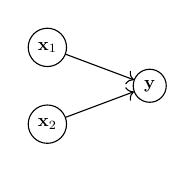
\begin{tikzpicture}[scale=.65, transform shape]
                \node[draw,circle] (x2) at (0,.75) {$\x_1$};
                \node[draw,circle] (x1) at (0,-.75) {$\x_2$};
                \node[draw,circle] (y) at (2,0) {$\y$};
                \draw [->] (x1) -- (y);
                \draw [->] (x2) -- (y);
            \end{tikzpicture}
            }
            \hspace{.3in}
            \subfigure[BC]{
              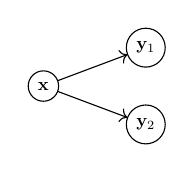
\begin{tikzpicture}[scale=.65, transform shape]
                \node[draw,circle] (y2) at (2,.75) {$\y_1$};
                \node[draw,circle] (y1) at (2,-.75) {$\y_2$};
                \node[draw,circle] (x) at (0,0) {$\x$};
                \draw [->] (x) -- (y1);
                \draw [->] (x) -- (y2);
            \end{tikzpicture}
            }
            \hspace{.3in}
            \subfigure[IC]{
              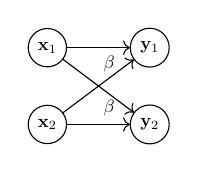
\begin{tikzpicture}[scale=.65, transform shape]
                \node[draw,circle] (x1) at (0,.75) {$\x_1$};
                \node[draw,circle] (x2) at (0,-.75) {$\x_2$};
                \node[draw,circle] (y1) at (2,.75) {$\y_1$};
                \node[draw,circle] (y2) at (2,-.75) {$\y_2$};
                \draw [->] (x1) -- (y1);
                \draw [->] (x1) -- node[anchor=north,pos=0.65] {$\beta$} (y2);
                \draw [->] (x2) -- node[anchor=south,pos=0.65] {$\beta$} (y1);
                \draw [->] (x2) -- (y2);
            \end{tikzpicture}
            }
            \hspace{.3in}
            \subfigure[RC]{
              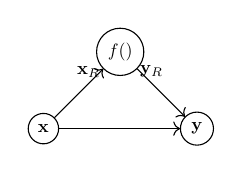
\begin{tikzpicture}[scale=.65, transform shape]
                \node[draw,circle] (x) at (0,-.75) {$\x$};
                \node[draw,circle] (r) at (1.5,.75) {$f()$};
                \node[draw,circle] (y) at (3,-.75) {$\y$};
                \draw [->] (x) -- (y);
                \draw [->] (x) -- node[anchor=south,pos=.7] {$\x_R$} (r);
                \draw [->] (r) -- node[anchor=south,pos=.3] {$\y_R$} (y);
            \end{tikzpicture}
            }
            \hspace{.3in}
            \subfigure[Two-Way]{
              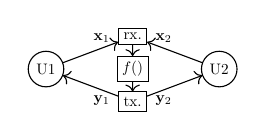
\begin{tikzpicture}[scale=.55, transform shape]
                \node[draw,circle] (u1) at (0,0) {U1};
                \node[draw,circle] (u2) at (4,0) {U2};
                \node[draw,rectangle] (rx) at (2,.75) {rx.};
                \node[draw,rectangle] (fx) at (2,0) {$f()$};
                \node[draw,rectangle] (tx) at (2,-.75) {tx.};
                \draw [->] (u1) -- node[anchor=south,pos=.7] {$\x_1$} (rx);
                \draw [->] (u2) -- node[anchor=south,pos=.7] {$\x_2$} (rx);
                \draw [->] (tx) -- node[anchor=north,pos=.3] {$\y_1$} (u1);
                \draw [->] (tx) -- node[anchor=north,pos=.3] {$\y_2$} (u2);
                \draw [->] (rx) -- (fx);
                \draw [->] (fx) -- (tx);
            \end{tikzpicture}
            }
            \hspace{.3in}
            \subfigure[Arbitrary Graph]{
              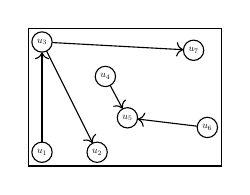
\begin{tikzpicture}[scale=.35, transform shape]
              \draw (-.5,-.5) rectangle (6.5,4.5);
                \node[draw,circle] (u1) at (0,0) {$u_1$};
                \node[draw,circle] (u2) at (2,0) {$u_2$};
                \node[draw,circle] (u3) at (0,4) {$u_3$};
                \node[draw,circle] (u4) at (2.3,2.75) {$u_4$};
                \node[draw,circle] (u5) at (3.1,1.25) {$u_5$};
                \node[draw,circle] (u6) at (6,.9) {$u_6$};
                \node[draw,circle] (u7) at (5.5,3.7) {$u_7$};                
                \draw [->] (u1) -- (u3);
                \draw [->] (u3) -- (u7);
                \draw [->] (u3) -- (u2);
                \draw [->] (u4) -- (u5);
                \draw [->] (u6) -- (u5);
            \end{tikzpicture}
            }
            
            \end{figure}


    \begin{itemize}
     \item MAC and BC are \textbf{simple cases}, most shapes are unsolved\\ \ \\
     \item We only have \textbf{bounds} (ex. CSB) and \textbf{limits} (ex. DoF)\\ \ \\
    \end{itemize} 
    }
    
    
\frame[allowframebreaks]{\frametitle{SISO Gaussian Interference Channel}
        \begin{figure}         
              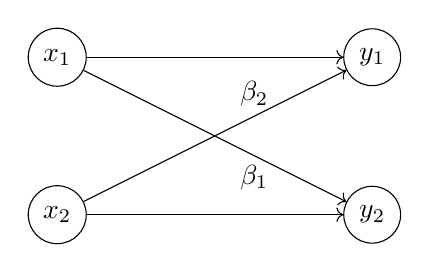
\begin{tikzpicture}[scale=1, transform shape]
                \node[draw,circle] (x1) at (0,1) {$x_1$};
                \node[draw,circle] (x2) at (0,-1) {$x_2$};
                \node[draw,circle] (y1) at (4,1) {$y_1$};
                \node[draw,circle] (y2) at (4,-1) {$y_2$};
                \draw [->] (x1) -- (y1);
                \draw [->] (x1) -- node[anchor=north,pos=0.65] {$\beta_1$} (y2);
                \draw [->] (x2) -- node[anchor=south,pos=0.65] {$\beta_2$} (y1);
                \draw [->] (x2) -- (y2);
            \end{tikzpicture}
        \end{figure}        
        $$y_i=x_i+\beta_{\textnormal{not}-i} x_{\textnormal{not}-i} +z_i$$
        \begin{itemize}
         \item  $\beta_{\{1,2\}}\in\mathbb{R}^+$: normalized to simplify notation\\ \ \\
         \item Looks very simple but is unsolved!\\ \ \\
        \end{itemize}
        }

\frame[allowframebreaks]{\frametitle{Weak Interference}
    \begin{lemma}[Outer Bound with Weak Interference ]
     If $\beta_2\frac{P_1}{BN_o}+\beta_1\frac{P_2}{BN_o}<\frac{1-\beta_2-\beta_2}{\beta_1\beta_2}$ then
     $$R_1+R_2\leq \log\left(1+\frac{P_1}{\beta_2^2P_2+BN_o}\right)+\log\left(1+\frac{P_2}{\beta_1^2P_1+BN_o}\right)$$
     \end{lemma}
     \begin{theorem}
       Treating Interference as Noise (TIN) is optimal with WI
       $$R_i^{TIN}= \log\left(1+\frac{P_i}{\beta_{\textnormal{not}-i}^2P_{\textnormal{not}-i}+BN_o}\right)$$
     \end{theorem}
     \begin{itemize}
      \item \textcolor{ARust}{Remember optimal in capacity $\neq$ good BER with QAM}
     \end{itemize}

}


\frame[allowframebreaks]{\frametitle{Very Strong Interference}
    \begin{theorem}[Very Strong Interference ]
     With the condition ``User 1 can decode $\beta_2 x_2$ treating $x_1$ as noise''
        $$\log\left(1+\frac{\beta_2P_2}{BN_o+P_1}\right)>\log\left(1+\frac{P_1}{BN_o}\right)$$ then 
        $$R_1= \log\left(1+\frac{P_1}{BN_o}\right)$$
     \end{theorem}
     \begin{itemize}
      \item User 1 can behave as MAC: cancel  $\beta_2 x_2$ to decode $x_1$\\ \ \\
      \item Very strong $\frac{\beta_2P_2}{BN_o}>\left(1+\frac{P_1}{BN_o}\right)\frac{P_1}{BN_o}>\left(\frac{P_1}{BN_o}\right)^2$
     \end{itemize}    
}


\frame[allowframebreaks]{\frametitle{Interference Channels in Practice}
    \begin{itemize}
     \item Tx. and rx. \textbf{can not connect}
     \begin{itemize}
     \item Example: Multiple satellites in the same band \\ \ \\
     \end{itemize}
     \item Joint en/de-coding is too \textbf{expensive}
     \begin{itemize}
     \item Example: Large mobile cellular networks\\ \ \\
     \end{itemize}
     \item Owners do not agree because \textbf{politics}
     \begin{itemize}
     \item Example: Opportunistic Cognitive Radio
     \end{itemize}
    \end{itemize}
    \vspace{-.1in}
\begin{figure}
 \centering
 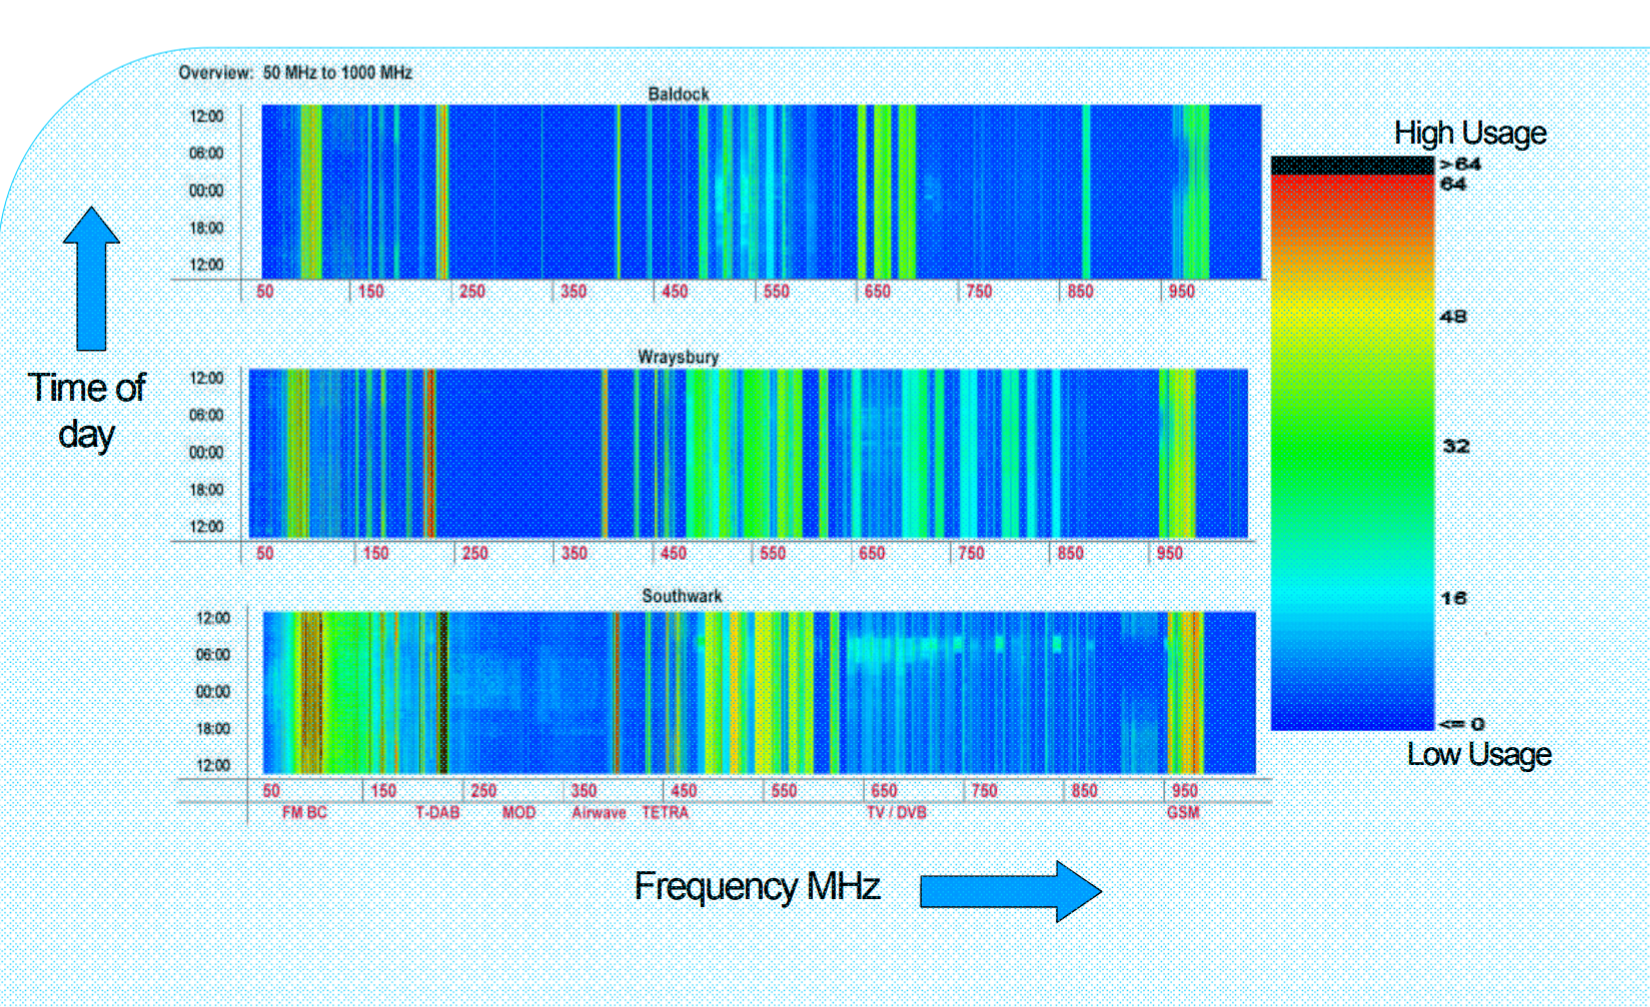
\includegraphics[width=.45\columnwidth]{whitespaces}
%  \caption{Spectrum use in rural/airport/metropolitan areas (Ofcom)}
\end{figure}
}
        
\frame[allowframebreaks]{\frametitle{Interference in Cellular Networks}
\begin{definition}[Path Loss Exponent $\alpha$]
 In radio propagation received power is $P_{rx}\approx P_{tx}d^{-\alpha}$ with $\alpha\geq 2$
\end{definition}

$$R_{i,j}\simeq B\log_2\left(1+\frac{d_{i,j}^{-\alpha}P_{tx,i}}{BN_o+\sum_{(n,m)\neq (i,j)}d_{n,j}^{-\alpha}P_{tx,n}}\right)\to \beta_{i,j}\propto \left(\frac{d_{i,j}}{d_{n,j}}\right)^{\alpha}$$

\begin{figure}
\setcounter{subfigure}{0}
\subfigure[F. Reuse $1/3$]{
    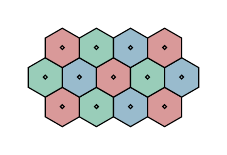
\begin{tikzpicture} [scale=.5, transform shape,hexa/.style= {shape=regular polygon,regular polygon sides=6,minimum size=1cm, draw,inner sep=0,anchor=south,rotate=30}]
    \foreach \j in {-1,...,1}{%            
    \foreach \i in {-2,...,2}{%
    \pgfmathparse{int(\i*\j)}
        \ifthenelse{\pgfmathresult=-2}{}{
        \pgfmathparse{int(Mod(\i+\j,3))}
            \ifthenelse{\pgfmathresult=0}{
                \node[hexa,fill=ARust!40] (\i;\j) at ({(\i-\j/2)*sin(60)},{\j*0.75}) {};
                \node[draw,circle, inner sep=1,minimum size=.1] at ({(\i-\j/2)*sin(60)-.22},{\j*0.75+.39}) {};
            }{}
            \ifthenelse{\pgfmathresult=1}{
                \node[hexa,fill=KYJade!40] (\i;\j) at ({(\i-\j/2)*sin(60)},{\j*0.75}) {};
                \node[draw,circle, inner sep=1,minimum size=.1] at ({(\i-\j/2)*sin(60)-.22},{\j*0.75+.39}) {};
            }{}
            \ifthenelse{\pgfmathresult=2}{
                \node[hexa,fill=VCobalt!40] (\i;\j) at ({(\i-\j/2)*sin(60)},{\j*0.75}) {};
                \node[draw,circle, inner sep=1,minimum size=.1] at ({(\i-\j/2)*sin(60)-.22},{\j*0.75+.39}) {};
            }{}
          }
        }   
    }            
    \end{tikzpicture}
    }
            \hspace{.4in}
\subfigure[F. Reuse $1$]{
    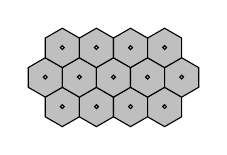
\begin{tikzpicture} [scale=.5, transform shape,hexa/.style= {shape=regular polygon,regular polygon sides=6,minimum size=1cm, draw,inner sep=0,anchor=south,rotate=30}]
    \foreach \j in {-1,...,1}{%            
    \foreach \i in {-2,...,2}{%
    \pgfmathparse{int(\i*\j)}
        \ifthenelse{\pgfmathresult=-2}{}{
            \node[hexa,fill=gray!50] (\i;\j) at ({(\i-\j/2)*sin(60)},{\j*0.75}) {};
            \node[draw,circle, inner sep=1,minimum size=.1] at ({(\i-\j/2)*sin(60)-.22},{\j*0.75+.39}) {};
        }
        }   
    }            
    \end{tikzpicture}
    }
            \hspace{.4in}
    \subfigure[Cooperative Multi-Point]{
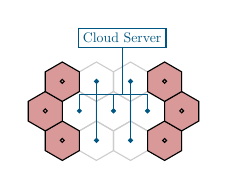
\begin{tikzpicture} [scale=.5, transform shape,hexa/.style= {shape=regular polygon,regular polygon sides=6,minimum size=1cm, draw,inner sep=0,anchor=south,rotate=30}]
    \node[rectangle,draw,color=VCobalt] (server) at (0,2.25) {Cloud Server};
    \coordinate (curb) at (0,.8);
    \foreach \j in {-1,...,1}{%            
    \foreach \i in {-2,...,2}{%
    \pgfmathparse{int(\i*\j)}
        \ifthenelse{\pgfmathresult=-2}{}{
            \node[hexa,color=gray!40] at ({(\i-\j/2)*sin(60)},{\j*0.75}) {};
            \node[circle,draw,color=VCobalt, fill=VCobalt, inner sep=1,minimum size=.1]  (\i;\j) at ({(\i-\j/2)*sin(60)-.22},{\j*0.75+.39}) {};
        }
        }   
    }
    \foreach \j in {-1,...,1}{%            
    \foreach \i in {-2,...,2}{%
    \pgfmathparse{int(\i*\j)}
        \ifthenelse{\pgfmathresult=-2}{}{
        \pgfmathparse{int(abs(\i))}
        \ifthenelse{ \pgfmathresult<2 }{ 
            \pgfmathparse{int(abs(\i-\j))}       
            \ifthenelse{ \pgfmathresult<2 }{
            \draw[color=VCobalt] (server) -- (curb) -|  (\i;\j);
            }{
                \node[hexa,fill=ARust!40] at ({(\i-\j/2)*sin(60)},{\j*0.75}) {};
                \node[circle,draw,color=black, inner sep=1,minimum size=.1]  (\i;\j) at ({(\i-\j/2)*sin(60)-.22},{\j*0.75+.39}) {};
            }
        }{
                \node[hexa,fill=ARust!40] at ({(\i-\j/2)*sin(60)},{\j*0.75}) {};
                \node[circle,draw,color=black, inner sep=1,minimum size=.1]  (\i;\j) at ({(\i-\j/2)*sin(60)-.22},{\j*0.75+.39}) {};
            }            
        }{}
        }   
    } 
                 
    \end{tikzpicture}
    }
\end{figure}
\vspace{-.2in}
\begin{columns}
 \begin{column}{3.5cm}
    \begin{itemize}
        \item Bandwidth $B/3$ 
        \item $\beta\propto (\sqrt{3}d_{\min})^{-\alpha}$
   \end{itemize}
 \end{column}
 \begin{column}{3.5cm}
    \begin{itemize}
        \item Bandwidth $B$ 
        \item $\beta\propto d_{\min}^{-\alpha}$
   \end{itemize}  
 \end{column}
 \begin{column}{4cm}
    \begin{itemize}
        \item Bandwidth $B$ 
        \item Becomes MAC/BC
   \end{itemize}
  
 \end{column}
\end{columns}
}

\frame[allowframebreaks]{\frametitle{\small Homework: Cooperative Multi-Point (CoMP)}
% \begin{homework}
 Consider the CoMP system in Fig. \ref{fig:comp}. There are two mobile towers at different locations acting as two SISO receivers and there are 2 users acting as transmitters, one near each tower. 
Each receiver $i$ sees the channel 
    $$y_i=h_{1,i}x_1+h_{2,i}x_2+z_i$$ 
    
    \begin{figure}[h]
    \centering
        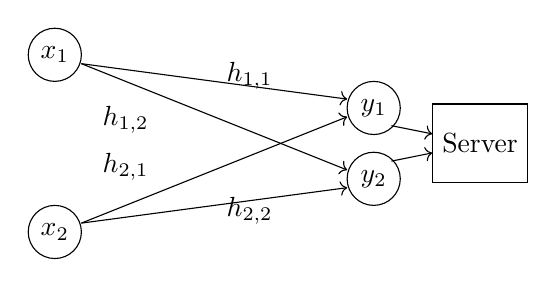
\begin{tikzpicture}[scale=.45]
            \draw [->] (.75,2.25) -- (8.25,1.25);
            \draw [->] (.75,-2.25) -- (8.25,-1.25);
            \draw [->] (.75,2.25) -- (8.25,-.75);
            \draw [->] (.75,-2.25) -- (8.25,.75);
            \node at (0,2.5) {$x_1$};
            \node at (0,-2.5) {$x_2$};
            \draw (9,1) circle (.75);
            \draw (0,2.5) circle (.75);
            \draw (9,-1) circle (.75);
            \draw (0,-2.5) circle (.75);
            \node[block] (server) at (12,0) {Server};
            \draw[->] (9.5,.5) -- (server);
            \draw[->] (9.5,-.5) -- (server);
            \node at (9,1) {$y_1$};
            \node at (9,-1) {$y_2$};
    %                 \draw (6,0) ellipse (1 and 2.5) dashed;
            \node[anchor=south] at (5.5,1.25) {$h_{1,1}$};
            \node[anchor=south] at (2,0) {$h_{1,2}$};
            \node[anchor=north] at (2,0) {$h_{2,1}$};
            \node[anchor=north] at (5.5,-1.25) {$h_{2,2}$};
        \end{tikzpicture}
        \caption{A CoMP $2$-antenna SIMO MAC channel}
        \label{fig:comp}
     \end{figure}
% \end{homework}

\pagebreak
     \begin{itemize}
      \item In \textbf{standalone} mode, receiver $1$ decodes $x_1$ treating $h_{2,1}x_2$ as noise and assuming $h_{2,1}x_2\sim\mathcal{CN}(0,|h_{2,1}|^2P_2)$, and vice-versa.
      \item In \textbf{CoMP} mode, both receivers send $y_1$ and $y_2$ to the cloud server. The server creates $\y=(y_1,y_2)^T$ and decodes $x_1$ and $x_2$ using SIC. \\ \ \\
     \end{itemize}
     
     \begin{enumerate}
      \item Write the MIMO DEC for the CoMP case using $\x=(x_1,x_2)^T$.
      \item Write the SINR for both cases
      \item Write a sum-rate expression in both cases
      \item Show that $R_1^{standalone}+R_2^{standalone}\leq R_1^{CoMP}+R_2^{CoMP}$ (Hint: use the chain rule)
     \end{enumerate}
}

\frame[allowframebreaks]{\frametitle{Practical Network Analysis}
 \begin{itemize}
\begin{columns}
\begin{column}{6cm}
        \item IT assumptions $\neq$ practical network
        \begin{itemize}
            \item Bursty traffic  \& queues\\ \ \\
            \item Variable user population\\ \ \\
            \item Decentralized networks\\ \ \\
            \item Asynchronous operations
        \end{itemize}
\end{column}
\begin{column}{6cm}
\begin{figure}
    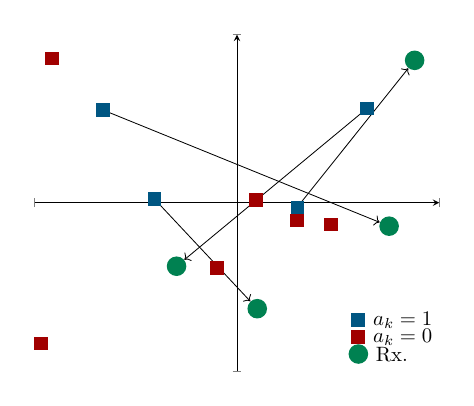
\begin{tikzpicture}[scale=.75]
        \tikzset{mark options={mark size=3}}
        \begin{axis}[
            axis x line=center,
            axis y line=center,
            xmin=-1,xmax=1,
            ymin=-1, ymax=1,
            xtick={-1,...,1},
            xticklabels={,,},
            ytick={-1,...,1},
            yticklabels={,,},
            scatter/classes={%
            a={mark=square*,color=VCobalt},
            b={mark=square*,color=ARust},
            c={mark=*,color=black}}]

            \addplot[scatter,only marks,%
                scatter src=explicit symbolic]%
                table[meta=label]{
                    x         y       label
                    0.6424    0.5605  a
                    0.2982    -0.0264 a
                    -0.6620   0.5514  a
                    -0.4074   0.0215  a
                    -0.0982   -0.3873 b
                    0.4634    -0.1283 b
                    -0.9692   -0.8377 b
                    -0.9140   0.8588  b
                    0.2955    -0.1064 b
                    0.0940    0.0170  b
            };
            \node[circle,fill=KYJade] (d1) at (axis cs: -0.2985 ,  -0.3778) {};
            \node[circle,fill=KYJade] (d2) at (axis cs: 00.8780 ,  0.8468) {};
            \node[circle,fill=KYJade] (d3) at (axis cs: 00.7519 ,  -0.1396) {};
            \node[circle,fill=KYJade] (d4) at (axis cs: 00.1003 ,  -0.6304 ) {};
            \draw [color=black,->] (axis cs: 0.6424,.5605) -- (d1);
            \draw [color=black,->] (axis cs: 0.2982,-.0264) -- (d2);
            \draw [color=black,->] (axis cs: -0.6620,.5514) -- (d3);
            \draw [color=black,->] (axis cs: -0.4074,.0215) -- (d4);        
            \node[rectangle,fill=VCobalt,label=right:{$a_k=1$}] at (axis cs: 0.6 ,  -0.7) {};
            \node[rectangle,fill=ARust,label=right:{$a_k=0$}] at (axis cs: 0.6 ,  -0.8) {};
            \node[circle,fill=KYJade,label=right:{Rx.}] at (axis cs: 0.6 ,  -.9) {};
        \end{axis}
        \end{tikzpicture}    
        \end{figure}
        
            \item Random activation with prob $p_a$
            \begin{itemize}
            \item $a_k=1$ if user $k$ active
            \item $a_k=0$ if not
         \end{itemize}
\end{column}
\end{columns}
\pagebreak
        \item Throughput Upper Bound for \textbf{symmetric} case $R_1=R_2\dots$
         \begin{itemize}
            \item Assume single user tx. and rx. 
            \item Assume all received power and interference are equal
            \item All users know the set of active users, CSI etc.
         $$T = \sum R_{k}\leq \sum_{n_a=1}^{K}{K \choose n_a}p_a^{n_a}(1-p_a)^{K-n_a}\log\left(1+\frac{KP}{\sigma^2p_a}\right)$$
        \end{itemize}

        \item Multi Packet Reception:         
         \begin{itemize}
            \item simultaneous $\tilde{k}$-user decoding in each rx.
         $$T_{MPR} = \sum R_{k}\leq \max_{\tilde{k}} \sum_{n_a=1}^{K}{K \choose n_a}p_a^{n_a}(1-p_a)^{K-n_a}\frac{n_a}{\tilde{k}}\log\left(1+\frac{\tilde{k}P}{\sigma^2p_a}\right)$$
        \end{itemize}
    \end{itemize}
}

\frame[allowframebreaks]{\frametitle{Interference vs Network Density}
\begin{enumerate}
 \item Interference Limited Network
 \begin{itemize}
    \item Very high user density,
    $$BN_o\ll\sum_{(n,m)\neq (i,j)}d_{n,j}^{-\alpha}P_{tx,n}$$
    \item SINR$\simeq$ SIR
    \begin{itemize}
    \item does not decrease if we increase DoF
    \item constant or decreases by increasing density\\ \ \\
    \end{itemize}
    \item ZF/SIC/MU-MIMO signal processing very beneficial\\ \ \\
    \item We can increase capacity buying spectrum and antennas $\to$ \circled{2}\\ \ \\
 \end{itemize}
 \pagebreak
 \item Noise Limited Network
 \begin{itemize}
    \item Low user density or very large bandwidth
    $$BN_o\gg\sum_{(n,m)\neq (i,j)}d_{n,j}^{-\alpha}P_{tx,n}$$
    \item SINR$\simeq$ SNR,
    \begin{itemize}
    \item decreases if we increase DoF
    \item always increases by increasing density\\ \ \\
    \end{itemize}
    \item TIN is optimal, hardware design simplified\\ \ \\
    \item We can increase capacity installing more devices $\to$ \circled{1}\\ \ \\
 \end{itemize}
\end{enumerate}

}

  
\frame[allowframebreaks]{\frametitle{Hybrid Automated Repeat reQuest (HARQ)}
\begin{columns}
 \begin{column}{8.5cm}  
    \begin{itemize}
     \item \textbf{Memorize} old failed transmissions\\ \ \\
     \item Effective rate $R=(1-P_{retx})R_{_{old}}+P_{retx}R_{retx}$\\ \ \\
     \item Diversity Combining:
     \begin{itemize}
     \item Same symbols in both transmissions $x_{_{new}}=x_{_{old}}$
     \item Equivalent SIMO channel
     $$\left(\begin{array}{c}
        y_{_{old}}\\
        y_{_{new}}
       \end{array}\right)
       =\left(\begin{array}{c}
        h_{_{old}}\\
        h_{_{new}}
       \end{array}\right)x+\z= \h x +\z$$
     \item Achieved rate
        $$R_{rtx}=\frac{1}{2}B\log_2\left(1+\frac{P\|\h_{eq}\|^2}{BN_o}\right)$$
    \end{itemize}

    \end{itemize}
 \end{column}
 \begin{column}{3cm}
  \begin{figure}
   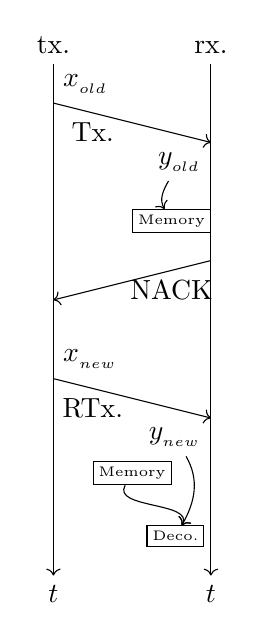
\begin{tikzpicture}
    \draw[->] (0,0)  -- node[anchor=north,pos=1] {$t$} node[anchor=south,pos=0] {tx.} (0,-6.5);
    \draw[->] (2,0) -- node[anchor=north,pos=1] {$t$} node[anchor=south,pos=0] {rx.} (2,-6.5);
    \draw[->] (0,-.5) -- node[anchor=north,pos=.25] {Tx.} node[anchor=south west,pos=0] {$x_{_{old}}$} node[anchor=north east,pos=1] (yold) {$y_{_{old}}$} (2,-1);
    \node[block,inner sep=2,minimum size=.1] (mem) at (1.5,-2) {\tiny Memory};
    \draw[->] (yold) to [in=120,out=-120] (mem);
    \draw[->] (2,-2.5) -- node[anchor=north,pos=.25] {NACK} (0,-3);
    \draw[->] (0,-4) -- node[anchor=north,pos=.25] {RTx.} node[anchor=south west,pos=0] {$x_{_{new}}$} node[anchor=north east,pos=1] (ynew) {$y_{_{new}}$} (2,-4.5);
    \node[block,inner sep=2,minimum size=.1] (mem2) at (1,-5.2) {\tiny Memory};
    \node[block,inner sep=2,minimum size=.1] (dec) at (1.55,-6) {\tiny Deco.};
    \draw[->] (ynew) to [in=60,out=-60] (dec);
    \draw[->] (mem2) to [in=60,out=-120] (dec);
   \end{tikzpicture}
  \end{figure}

 \end{column}
\end{columns}
\begin{columns}
 \begin{column}{8.5cm} 
    \begin{itemize}
     \item Incremental Redundancy:
     \begin{itemize}
     \item Independent codebooks $$\x=(x_{_{old}},x_{_{new}})^T\to f(\x)=f(x_{_{old}})f(x_{_{new}})$$
     \item Equivalent MIMO channel
     $$\left(\begin{array}{c}
        y_{_{old}}\\
        y_{_{new}}
       \end{array}\right)
       =\left(\begin{array}{cc}
        h_{_{old}}&0\\
        0&h_{_{new}}
       \end{array}\right)
       \left(\begin{array}{cc}
        x_{_{old}}\\
        x_{_{new}}
       \end{array}\right)+\z=\Hb \x + \z$$
     \item Achieved rate
        \begin{align*}
            R_{rtx}&=\frac{1}{2}\log_2\left|\I_2+\frac{P}{BN_o}\Hb\Sb_{\x}\Hb^H\right|\\
            &=\frac{1}{2}R_{_{old}}+\frac{1}{2}B\log_2\left(1+\frac{P}{BN_o}|h_{_{new}}|^2\right)
        \end{align*}
    \end{itemize}
    \end{itemize}
 \end{column}
 \begin{column}{3cm}
  \begin{figure}
   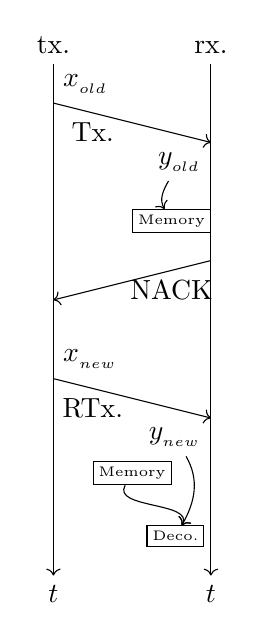
\begin{tikzpicture}
    \draw[->] (0,0)  -- node[anchor=north,pos=1] {$t$} node[anchor=south,pos=0] {tx.} (0,-6.5);
    \draw[->] (2,0) -- node[anchor=north,pos=1] {$t$} node[anchor=south,pos=0] {rx.} (2,-6.5);
    \draw[->] (0,-.5) -- node[anchor=north,pos=.25] {Tx.} node[anchor=south west,pos=0] {$x_{_{old}}$} node[anchor=north east,pos=1] (yold) {$y_{_{old}}$} (2,-1);
    \node[block,inner sep=2,minimum size=.1] (mem) at (1.5,-2) {\tiny Memory};
    \draw[->] (yold) to [in=120,out=-120] (mem);
    \draw[->] (2,-2.5) -- node[anchor=north,pos=.25] {NACK} (0,-3);
    \draw[->] (0,-4) -- node[anchor=north,pos=.25] {RTx.} node[anchor=south west,pos=0] {$x_{_{new}}$} node[anchor=north east,pos=1] (ynew) {$y_{_{new}}$} (2,-4.5);
    \node[block,inner sep=2,minimum size=.1] (mem2) at (1,-5.2) {\tiny Memory};
    \node[block,inner sep=2,minimum size=.1] (dec) at (1.55,-6) {\tiny Deco.};
    \draw[->] (ynew) to [in=60,out=-60] (dec);
    \draw[->] (mem2) to [in=60,out=-120] (dec);
   \end{tikzpicture}
  \end{figure}

 \end{column}
\end{columns}
}

\frame[allowframebreaks]{\frametitle{Gaussian Relay Channel}

\begin{columns}
 \begin{column}{6cm}
   $$\y_R=\Hb_2\x+\z_R$$
    $$\x_R\sim f(\x_R|\y_R)$$
    $$\y=\Hb_1\x+\Hb_3\x_R+\z$$\\ \ \\
 \end{column}
 \begin{column}{6cm}
  \begin{figure}
        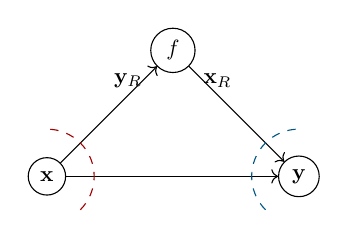
\begin{tikzpicture}[scale=.8, transform shape]
            \node[draw,circle] (x) at (0,-1) {$\x$};
            \node[draw,circle] (r) at (2,1) {$f$};
            \node[draw,circle] (y) at (4,-1) {$\y$};
            \draw [->] (x) -- (y);
            \draw [->] (x) -- node[anchor=south,pos=.7] {$\y_R$} (r);
            \draw [->] (r) -- node[anchor=south,pos=.3] {$\x_R$} (y);
            \draw [ARust,dashed,domain=-45:90] plot ({0+.75*cos(\x)}, {-1+.75*sin(\x)});
            \draw [VCobalt,dashed,domain=-45:90] plot ({4-.75*cos(\x)}, {-1+.75*sin(\x)});
        \end{tikzpicture}
    \end{figure}
    
  
 \end{column}
\end{columns}
  \begin{itemize}
   \item In general $\y$ includes a direct reception of $\x$\\ \ \\
   \item Cut-set Upper Bound \textbf{Not Tight!}  
   \begin{itemize}
    \item Optimize over all possible relations $f(\x_R|\y_R)$
   \end{itemize}
$$C\leq \sup_{f(\x_R|\y_R)}\min\left(\;\textcolor{ARust}{\underset{\textnormal{BC-cut}}{\underbrace{\CInf{(\y,\y_R)}{\x}{\Hb_1,\Hb_3,\x_R}}}},\;
                      \textcolor{VCobalt}{\underset{\textnormal{MAC-cut}}{\underbrace{\CInf{\y}{(\x_R,\x)}{\Hb_1,\Hb_2}}}}\;
                     \right)$$
\pagebreak
    \begin{definition}[Degraded Gaussian Relay Channel]
     If we can write $f(\y,\y_R|\x,\x_R)=f(\y_R|\x,\x_R)f(\y|\y_R,\x_R)$ the BC is \textbf{degraded} and the CSB is achievable. For the Gaussian case this happens with $\Hb_1=\zero$.
    \end{definition}
    
    \begin{definition}[Half Duplex Constraint]
    Most radios cannot transmit and receive at the same time due to self interference \\ \ \\
   \end{definition}
    \item Consider the time axis with causality constraint and write
    \begin{table}
    \begin{tabular}{r|ll}
        & Relay rx.ing at $n$ & Relay tx.ing at $n$\\ \hline 
        $\y_R[n]=$&$\Hb_2\x[n]+\z_R[n]$&$0$\\
        $\x_R[n]=$&$0$&$~f(\x_R[n]|\y_R[\textcolor{ARust}{n-1}],\y_R[\textcolor{ARust}{n-2}]\dots)$\\
        $\y[n]=$&$\Hb_1\x[n]+\z[n]$&$\Hb_1\x[n]+\Hb_3\x_R[n]+\z[n]$\\
        \end{tabular}
    \end{table}
    \item Some Gaussian SISO Half-Duplex RC $\frac{1}{2}$-static schemes:\\ \ \\
    \begin{itemize}
        \item Amplify and Forward: $x_R[n]=Ay_R[n-1]$
            $$\y_{eq}=\left(\begin{array}{c}h_1\\h_2A h_3\end{array}\right)x+\left(\begin{array}{c}\sigma \overline{z}[n-1]\\(\sigma+h_{3}A\sigma_R)\overline{z}[n]\end{array}\right)$$
            $$R_{AF}=\frac{1}{2}\log\left|\Sb_{\y_{eq}|x}^{-1}\Sb_{\y_{eq}}\right|=\frac{1}{2}\log\left(1+\textcolor{ARust}{\gamma_1}+\frac{\gamma_2\gamma_3}{1+\gamma_2+\gamma_3}\right)$$
        \item Decode and forward: $x_R[n]=\hat{x}[n-1]=\textnormal{decode}(y_R[n-1])$
            $$R_{DF}=\frac{1}{2}\min\left\{\log\left(1+\gamma_2\right),\log\left(1+\textcolor{ARust}{\gamma_1}+\gamma_3\right)\right\}$$
%     \item Amplify and Forward\\ \ \\
%     \item Decode And Forward\\ \ \\´
  \end{itemize}
  \pagebreak
    \item Some Gaussian SISO Half-Duplex RC dynamic schemes:\\ \ \\
    \begin{itemize}
        \item Opportunistic Relaying: only use RC if $\gamma_1<2^{R_{RC}}-1$
            $$R_{OR}=\begin{cases}\log\left(1+\gamma_1\right)& \;\gamma_1\geq 2^{R_{RC}}-1\\
                                  R_{RC}&\;\gamma_1< 2^{R_{RC}}-1
                     \end{cases} $$
                     
        \item Dynamic Decode and Forward:             
        \begin{itemize}
            \item Variable time-division $\delta$
            $$R_{DF}=\min\left\{\delta\underset{R_2}{\underbrace{\log\left(1+\gamma_2\right)}},(1-\delta)\underset{R_{\textcolor{ARust}{1,}3}}{\underbrace{\log\left(1+\textcolor{ARust}{\gamma_1}+\gamma_3\right)}}\right\}$$
            \item Optimized $\delta^*=\frac{R_{3}}{R_2+R_{\textcolor{ARust}{1,}3}}$
            $$R_{DF}=\frac{R_2R_{3}}{R_2+R_{\textcolor{ARust}{1,}3}}=\frac{1}{\frac{1}{R_2}+\frac{1}{R_{\textcolor{ARust}{1,}3}}}$$
        \end{itemize}
  \end{itemize}
  \pagebreak
  \item Adaptive Modulation and Coding
%     \begin{itemize}
%         \item Code can use \textbf{puncturing}
%         \item Channel Quality Indication (CQI) messages
%     \end{itemize}
    \begin{figure}
     \begin{tikzpicture}[scale=.6, transform shape]
      \node[input] (inbits) {};
      \node[block, right of=inbits, node distance=3.5cm] (amc) {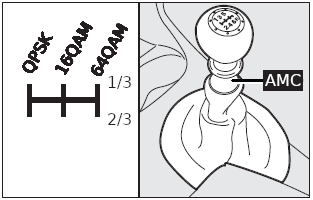
\includegraphics[width=4cm]{amc}};
      \draw [draw,->] (inbits) -- node[anchor=south] {$\bb_0,\bb_1\dots $} (amc);
      \node[block, right of=amc, node distance=3.5cm] (ch) {$\Hb$};
      \draw [draw,->] (amc) -- node[anchor=south] {$\x$} (ch);
      \node[block, right of=amc, node distance=3.5cm] (ch) {$\Hb$};
      \draw [draw,->] (amc) -- node[anchor=south] {$\x$} (ch);
      \coordinate[right of=ch,node distance=1.5cm] (probe);
      \draw [draw,-] (ch) -- node[anchor=south] {$\y$} (probe);
      \node[output,right of=probe,node distance=.5cm] (outsig) {};
      \draw [draw,->] (probe) -- (outsig);
      \node[block, below of=ch, node distance=2cm] (cqi) {CQI};
      \draw [draw,->] (probe) |- (cqi);
      \draw [draw,->] (cqi) -| (amc);
     \end{tikzpicture}
%      \caption{Adaptive Modulation and Coding}
    \end{figure}  
  
  \item \textbf{Shortest Total Transmission Time}
  
    \begin{itemize}
        \item Degraded Gaussian DF RC\\ \ \\
        \item Combines OR and DDF\\ \ \\
        \item Fixed message length $L$, tx. time is
        $$T=\min(T_{1},T_{2}+T_{3})=\min(\frac{L}{R_1},\frac{L}{R_2}+\frac{L}{R_3})\Leftrightarrow \max(R_1,\frac{R_2R_{3}}{R_2+R_{3}})$$
    \end{itemize}
    \pagebreak
    
  \begin{definition}[Two-Way Relaying]
    A two-user half-duplex RC can ``seem'' full-duplex.
  \end{definition}

  \begin{columns}
  \begin{column}{5cm}
   \begin{figure}
    \setcounter{subfigure}{0}
    \subfigure[t=1]{
    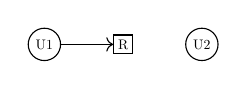
\begin{tikzpicture}[scale=.5,transform shape]
    \node[draw,circle] (A) at (0,0) {U1};
    \node[draw,rectangle] (R) at (2,0) {R};
    \node[draw,circle] (B) at (4,0) {U2};
    \draw[->] (A) -- (R);
    \end{tikzpicture}
   }
    \subfigure[t=2]{
    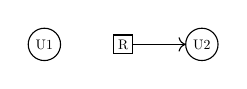
\begin{tikzpicture}[scale=.5,transform shape]
    \node[draw,circle] (A) at (0,0) {U1};
    \node[draw,rectangle] (R) at (2,0) {R};
    \node[draw,circle] (B) at (4,0) {U2};
    \draw[->] (R) -- (B);
    \end{tikzpicture}
   }
    \subfigure[t=3]{
    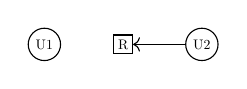
\begin{tikzpicture}[scale=.5,transform shape]
    \node[draw,circle] (A) at (0,0) {U1};
    \node[draw,rectangle] (R) at (2,0) {R};
    \node[draw,circle] (B) at (4,0) {U2};
    \draw[->] (B) -- (R);
    \end{tikzpicture}
   }
    \subfigure[t=4]{
    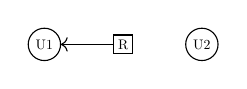
\begin{tikzpicture}[scale=.5,transform shape]
    \node[draw,circle] (A) at (0,0) {U1};
    \node[draw,rectangle] (R) at (2,0) {R};
    \node[draw,circle] (B) at (4,0) {U2};
    \draw[->] (R) -- (A);
    \end{tikzpicture}
   }
   \caption{Orthogonal 2-hop Duplex}
   \vspace{-.5in}
   \end{figure}
  \end{column}
  
  \begin{column}{5cm}
   \begin{figure}
   \setcounter{subfigure}{0}
    \subfigure[t=1]{
    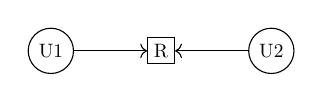
\begin{tikzpicture}[scale=.7,transform shape]
    \node[draw,circle] (A) at (0,0) {U1};
    \node[draw,rectangle] (R) at (2,0) {R};
    \node[draw,circle] (B) at (4,0) {U2};
    \draw[->] (A) -- (R);
    \draw[->] (B) -- (R);
    \end{tikzpicture}
   }
    \subfigure[t=2]{
    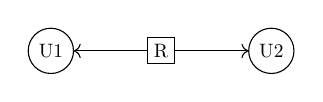
\begin{tikzpicture}[scale=.7,transform shape]
    \node[draw,circle] (A) at (0,0) {U1};
    \node[draw,rectangle] (R) at (2,0) {R};
    \node[draw,circle] (B) at (4,0) {U2};
    \draw[->] (R) -- (B);
    \draw[->] (R) -- (A);
    \end{tikzpicture}
   }
   \caption{Two-Way 2-hop Duplex}
   \end{figure}
  \end{column}   
  \end{columns}

  \end{itemize}
  }
  
\frame{\frametitle{Unsolved Capacity of Wireless Network}
\begin{figure}
    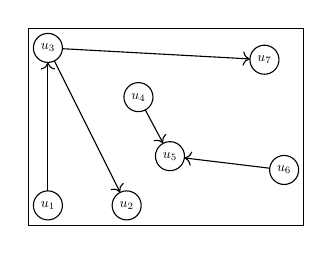
\begin{tikzpicture}[scale=.5, transform shape]
    \draw (-.5,-.5) rectangle (6.5,4.5);
    \node[draw,circle] (u1) at (0,0) {$u_1$};
    \node[draw,circle] (u2) at (2,0) {$u_2$};
    \node[draw,circle] (u3) at (0,4) {$u_3$};
    \node[draw,circle] (u4) at (2.3,2.75) {$u_4$};
    \node[draw,circle] (u5) at (3.1,1.25) {$u_5$};
    \node[draw,circle] (u6) at (6,.9) {$u_6$};
    \node[draw,circle] (u7) at (5.5,3.7) {$u_7$};                
    \draw [->] (u1) -- (u3);
    \draw [->] (u3) -- (u7);
    \draw [->] (u3) -- (u2);
    \draw [->] (u4) -- (u5);
    \draw [->] (u6) -- (u5);
\end{tikzpicture}
\end{figure}
    \begin{itemize}
        \item Not necessary to joint-decode everything (TIN)\\ \ \\ 
        \item More interference can be good! (very strong)\\ \ \\
        \item Not desirable to always use same path (OR)\\ \ \\
        \item More users can be free! (two-way)\\ \ \\        
        \item Transmitter Rate can be adapted (AMC, HARQ)
    \end{itemize}
}

\end{document}


